\section{Contribution: Évaluation comparative stricte}

\subsection{Motivation}

\begin{frame}{Motivation}

    Les résultats rapportés dans les articles ne sont \textbf{pas directement comparables}.
    
    %La différence de \textbf{jeux de données} et \textbf{métriques} utilisés ainsi que les \textbf{cadre expérimentaux} notamment les pré-traitements différents~ \cite{boudin_how_2016} rendent les scores peu comparables.
    
    \begin{block}{Incomparabilité causé par}
    \begin{enumerate}
        \item Jeux de données différents
        \item Métriques différentes
        \item Pré-traitements différents
    \end{enumerate}
    \end{block}
    
    
    Trois articles publiés à ACL 2017 ne partagent aucun jeu de données et aucune métrique:
    {\footnotesize
    \cite{meng_deep_2017},% Inspec ACM NUS SemEval-2010 KP20k;F@5,10
    \cite{florescu_positionrank:_2017}, %KDD, WWW, NUS; PRF@2,4,6,8,MRR
    \cite{teneva_salience_2017} %KPCrowd Inspec PRF
    }
    
    \alt<2>{
    $\Rightarrow$ \'Evaluation à l'aide d'un cadre expérimental \textbf{strict} et \textbf{unifié}.}{\phantom{un texte très long sur deux lignes lalalalalalaalalalal deux lignes}}
\end{frame}

\iffalse
\begin{frame}{Motivation}
    %Pour obtenir un aperçu des performances des méthodes et indiquer quelles sont les méthodes à utiliser
    Nous évaluons 9 méthodes sur 9 jeux de données.

    \begin{block}{Cadre expérimental strict et partagé}
    \begin{enumerate}
        \item Pré-traitement
        \item Protocole d'évaluation
        \item Réimplémentation
    \end{enumerate}
    \end{block}
\end{frame}
\fi

\subsection{Cadre expérimental}

\begin{frame}<1>[label=aa]{Méthodes évaluées}
%\begin{columns}
%\begin{column}{0.5\textwidth}
    \begin{block}{Méthodes de base}
    \begin{itemize}
        \item FirstPhrases
        \item \textbf<2>{TextRank}~\cite{mihalcea_textrank:_2004}
        \item \textbf<2>{\tfidf{}}~\cite{jones_statistical_1972}
    \end{itemize}
    \end{block}
        
    \begin{block}{Méthodes non supervisées}
    \begin{itemize}
        \item PositionRank~\cite{florescu_positionrank:_2017}
        \item \textbf<3>{MultiPartiteRank}~\cite{boudin_unsupervised_2018}
        \item \textbf<4>{EmbedRank}~\cite{bennani-smires_simple_2018}
    \end{itemize}
    \end{block}
        
    \begin{block}{Méthodes supervisées}
    \begin{itemize}
        \item Kea~\cite{witten_kea:_1999}
        \item CopyRNN~\cite{meng_deep_2017}
        \item CorrRNN~\cite{chen_keyphrase_2018}
    \end{itemize}
    \end{block}
%\end{column}
%\begin{column}{0.5\textwidth}
    \begin{center}
     \only<2>{
     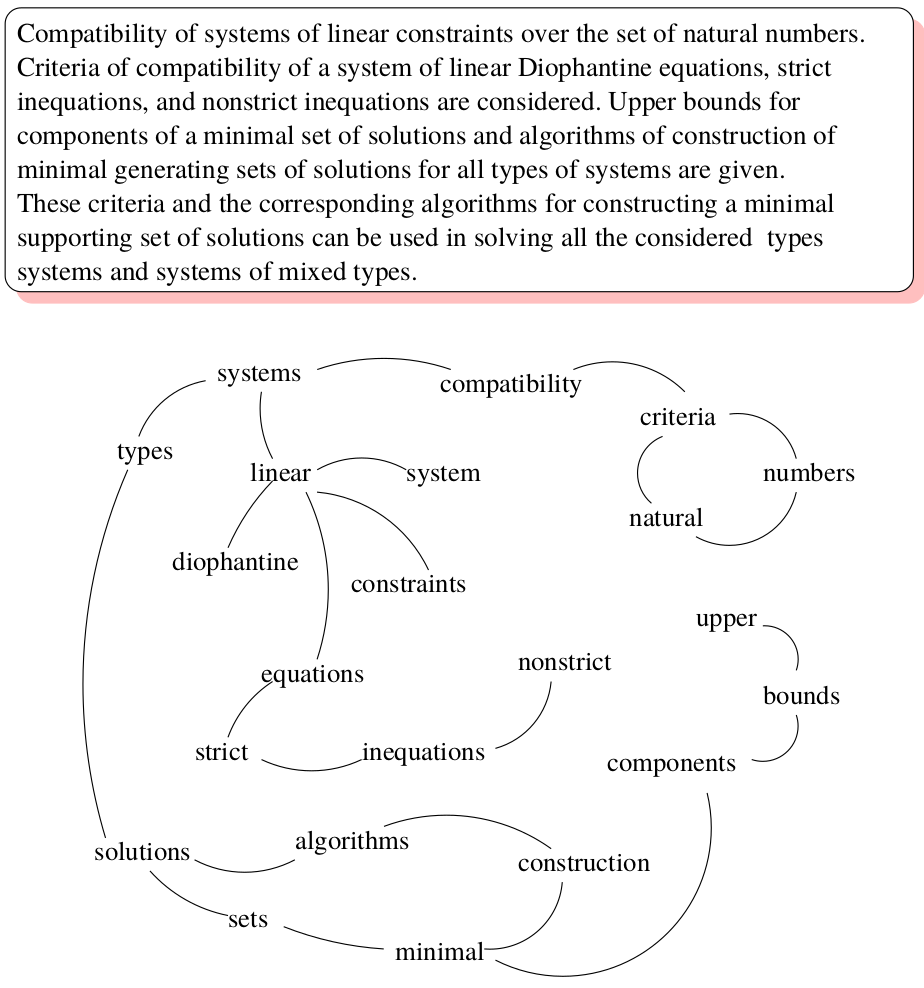
\includegraphics[width=0.9\textwidth,trim={0 0 0 32em},clip]{figures/large_textrank.png}}
     \only<2>{
     \begin{align*}
        \tfidf & (d, w) = \\
        & \textsc{Tf}_d(w) * log\left( \frac{N}{\textsc{Df}(w)} \right)
    \end{align*}
     }
     \only<3>{
     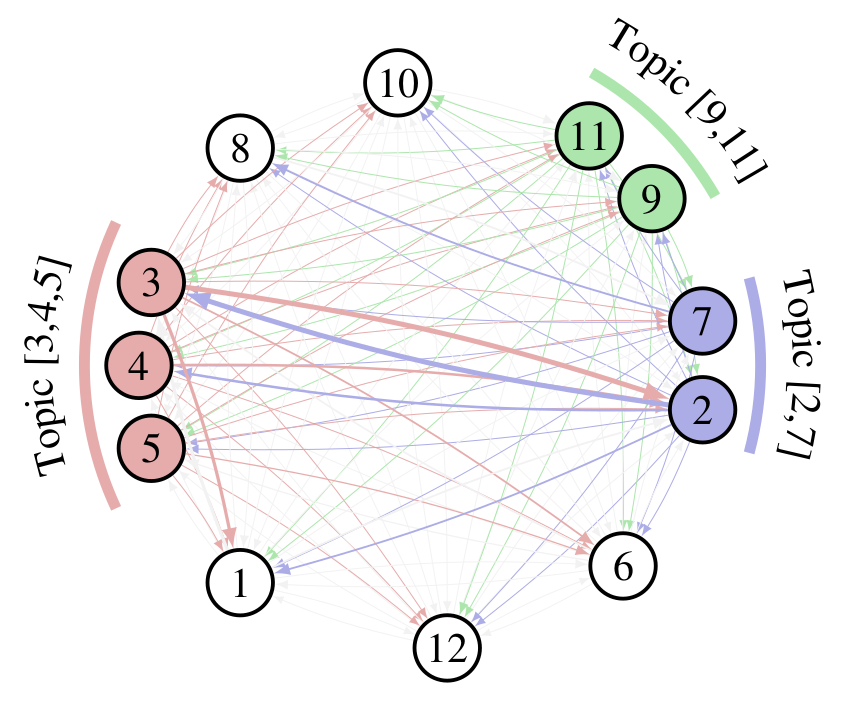
\includegraphics[width=0.9\textwidth]{figures/large_mprank.png}}
     \only<4>{
     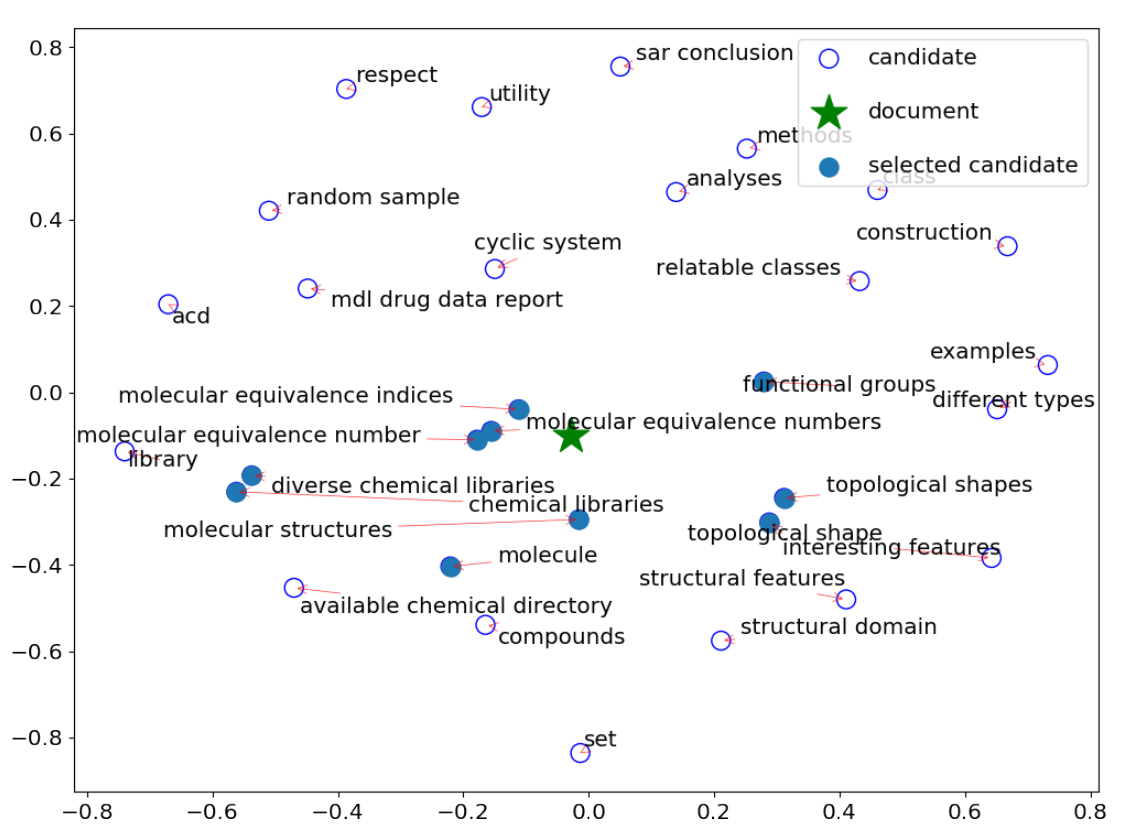
\includegraphics[width=1\textwidth]{figures/large_embedrank.png}}
     \end{center}
%\end{column}
%\end{columns}
\end{frame}

\begin{frame}{Jeux de données}
    %\newcommand{\tikzmark}[1]{%  \tikz[overlay,remember picture] \node (#1) {};}

%https://tex.stackexchange.com/a/6250/240347
%\alt<3>{\newcolumntype{C}{>{\columncolor{color1!40}}r}}{\newcolumntype{C}{r}}

\begin{table}[htbp!]
\centering
\resizebox{0.9\textwidth}{!}{
    \begin{tabular}{crcccrrrr}
    \cmidrule[1pt]{2-9}
        &
        \textbf{Corpus} &
        \textbf{Lang.} &
        \textbf{Ann.} &
        \textbf{\#Entr.} &
        \textbf{\#Test} &
        \textbf{\#mots} 
        & \textbf{\#mc} & \textbf{\%abs} \\

    \cmidrule[.5pt]{2-9}
    %\tikzmark{b}
    %& \cellcolor<3>{color1!40} CSTR~\cite{witten_kea:_1999}              & en & $A$        & \cellcolor<3>{color1!40} 130 & 500 &11501  & 5 & 19 \\
    %& NUS~\cite{goh_keyphrase_2007}             & en & $A \cup L$ & -   & 211 & 8398  &11 & 14 \\
    & PubMed~\cite{schutz_keyphrase_2008}       & en & $A$        & -   & 1320& 5323  & 5 & 17 \\
    & ACM~\cite{krapivin_large_2009}            & en & $A$        & -   & 2304& 9198  & 5 & 16 \\
    \multirow{-5}{*}[-0.4ex]{\rotatebox{90}{\textbf{Articles}}}
    %& Citeulike-180~\cite{medelyan_human-competitive_2009} & en & $L$ & -&182 & 8590  & 5 & 11 \\
    & SemEval-2010~\cite{kim_semeval-2010_2010} & en & $A \cup L$ & 144 & 100 & 7961  &15 & 20 \\
    
    %\cmidrule{7-9} %\vspace{-.5em}
    %\multirow{-6}{*}[-0.4ex]{\rotatebox{90}{\textbf{Articles}}}
    %& & & & & \textbf{Avg.} & 8495  & 8  & 16 \\
    
        \cmidrule[.5pt]{2-9}
    
    %\tikzmark{a}
    & Inspec~\cite{hulth_improved_2003}         & en & $I$ & 1\,000  & 500    & 135  & 10 & 22 \\
    %& KDD~\cite{caragea_citation-enhanced_2014} & en & $A$ & -       & 755    & 191  &  4 & 49 \\
    & WWW~\cite{caragea_citation-enhanced_2014} & en & $A$ & -       & 1\,330 & 164  &  5 & 52 \\
    %& TermITH-Eval~\cite{bougouin_termith-eval:_2016} & fr & $I$ & - & 400    & 165  & 12 & 60 \\
    \multirow{-5}{*}[-0.4ex]{\rotatebox{90}{\textbf{Notices}}}
    & KP20k~\cite{meng_deep_2017}               & en & $A$ & 530\,K  & 20\,K  & 176  &  5 & 43 \\
    %OAGK~\cite{cano_keyphrase_2019-1}         & en & $A$ & 23\,M   & -      & ?   & ?    & ? \\
    %\cmidrule{7-9} %\vspace{-.5em}
    %\multirow{-6}{*}[-0.4ex]{\rotatebox{90}{\textbf{Notices}}}
    %& & & & & \textbf{Avg.} & 166  & 7  & 45 \\
    
    \cmidrule[.5pt]{2-9}
    %Reuters-21578~\cite{hulth-megyesi:2006:COLACL}     & en & \\
    %110-PT-BN-KP~\cite{marujo_keyphrase_2011} & pt & $L$ & 100 & 10 & 439 & 27.6 & 7.5 \\
    & DUC-2001~\cite{wan_single_2008}            & en & $L$ & -    & 308 & 847  &  8 &  4 \\
    & 500N-KPCrowd~\cite{marujo_supervised_2012} & en & $L$ & 450  &  50 & 465  & 46 & 11 \\
    \multirow{-4}{*}[-0.4ex]{\rotatebox{90}{\textbf{Journalistiques}}}
    %& Wikinews~\cite{bougouin_topicrank:_2013}   & fr & $L$ & -    & 100 & 314  & 10 & 11 \\
    %\rowcolor<3>{color1!40}
    & KPTimes~\cite{gallina_kptimes_2019}        & en & $E$ &260\,K&20\,K& 784  &  5 & 41 \\

    %\cmidrule{7-9} %\vspace{-.5em}
    %\multirow{-5}{*}[-0.4ex]{\rotatebox{90}{\textbf{Journalistique}}}
    %& & & & & \textbf{Avg.} & 603  & 17  & 17 \\
    \cmidrule[1pt]{2-9}
    \end{tabular}
    
    %\tikz[right=5cm,overlay,remember picture] \node[rotate=90, anchor=center] at ($(a)!0.5!(b)$) {Notices};
    %\tikz[overlay,remember picture] \draw[-triangle 45] ($(a.north east)+(-0.2,0.2)$) -- ($(b.south west)+(0.3,-0.2)$);
}
%\caption{\footnotesize Statistiques des jeux de données de production automatique de mots-clés.
%Les mots-clés de référence sont annotés par les auteurs ($A$) ou des indexeurs professionnels ($I$).
%La table présente le nombre de documents dans les corpus d'entraînement (\#Entr.) et de test (\#Test) ainsi que le nombre moyen de mots-clés (\#mc), de mots (\#mots) et le ratio de mots-clés absent (\%abs) par document.}
%\label{tab:datasets_abstract}
\end{table}
    \begin{itemize}
        \item Représentatifs des jeux de données utilisés
        %\item Trois types de documents
        \item Différents types d'annotation (Auteur, Lecteur, Indexeur, \'Editeur)
    \end{itemize}
\end{frame}

\begin{frame}{Cadre expérimental strict}
    \begin{block}{Paramètres expérimentaux unifiés}
    \begin{itemize}
        \item \textbf{Prétraitements}: réalisé avec Stanford CoreNLP.
        \item \textbf{Sélection des candidats}: syntagmes nomimaux (\texttt{A*N+}) + filtrage. % mots courts, moins de 5 mots, non alpha, mots-vides
        \item \textbf{Métrique}: F@10
        
        \item \textbf{Entraînement}:
        \begin{itemize}
            \item Kea: en validation croisée si pas de documents d'entraînement.
            \item Méthodes génératives: sur KP20k et KPTimes en fonction du genre de document.
        \end{itemize}

        \item Utilisation des paramètres recommandés par les auteurs dans les articles originaux.
    \end{itemize}
    \end{block}
\end{frame}

\begin{frame}{Cadre expérimental strict}
    \begin{block}{Réimplémentation}
    
        Est-ce que nos réimplémentations obtiennent des résultats comparables aux méthodes originales ?
    
        \begin{table}[!htb]
    \centering
    \resizebox{\textwidth}{!}{
    \begin{tabular}{lrlccc}
    \toprule
    \textbf{Méthode} & \textbf{Jeu de données} & \textbf{Métrique} & \textbf{Orig.} & \textbf{Réimp.} & \textbf{Diff.} \\
    \midrule
        %Kea & \small{CSTR (matches@10)}          & 1,39 & 1,03 \\
        PositionRank & \small{WWW} & \small{F$@$8}       & 12,3 & 11,7 & \cellcolor{color1!40} -0,6 \\%[.3em]
        %PositionRank & \small{KDD (F$@$8)}       & 12,1 & 11,8 \\
        %TopicCoRank & \small{TermITH (F$@$10)}   & 20,4 & 19,5 \\
        MPRank & \small{SemEval-2010} & \small{F$@$10}   & 14,5 & 14,3 & \cellcolor{color1!40} -0,2 \\
        %     ~ & \small{Inspec (F$@$10)}         & 30,6 & 30,5 \\
        %     ~ & \small{KPCrowd (F$@$10)}        & 18,2 & 18,2 \\
        EmbedRank & \small{Inspec} & \small{F$@$10}   & 37,1 & 35,6  & \cellcolor{color1!40} -1,5 \\ % 36,3
        %       ~ & \small{DUC (F$@$10)}   & 31,9 & 29,5 \\ % 30,9
        %       ~ & \small{NUS (F$@$10)}   & \phantom{0}5,4 & 3,2 \\ % 5,2
        CopyRNN & \small{KP20k} & \small{F$@$10 (prs.)} & 26,2 & 28,2 & \cellcolor{color1!40} +2 \\
        %     ~ & \small{Inspec (F$@$10 present)} & 34,2 & 30,6 \\
        %     ~ & \small{SemEval (F$@$10 present)} & 30,4 & 23,0 \\
        CorrRNN & \small{ACM} & \small{F$@$10 (prs.)} & 27,8 & 24,7 & \cellcolor{color1!40} -3,1 \\ % (-3,1)
        %     ~ & \small{NUS (F$@$10 present)} & 33,0 & 26,8 (-6,2) \\
        %     ~ & \small{SemEval (F$@$10 present)} & 32,0 & 22,3 \\ % (-9,7)
    \bottomrule
    \end{tabular}
    }
    %\caption{Comparaison des scores des méthodes que nous avons réimplémentés avec les scores qui ont été rapportés dans les articles originaux.}
\end{table}

% KEA CSTR Avg. Matches @ 10 1.39 
        
        \begin{itemize}
        \item Résultats comparables
            \item Différences liées aux paramètres peu explicités
            %\item EmbedRank: différence liée à la casse
            %\item CopyRNN: ?
            %\item CorrRNN: différence d'entraînement (données)
        \end{itemize}
    \end{block}
\end{frame}

\section*{Analyse des résultats}

\begin{frame}{}
    \sectionpage
\end{frame}

\begin{frame}{Résultats généraux}
    \begin{table}
    \centering
    %\rotatebox{90}{%
    \resizebox{\linewidth}{!}{
\begin{tabular}{r c c c | c c c | c c c}
         &
        \multicolumn{3}{c}{\textit{Articles scientifiques}} &
        \multicolumn{3}{c}{\textit{Notices scientifiques}} &
        \multicolumn{3}{c}{\textit{Articles journalistiques}}
        \\
        
        \cmidrule(lr){2-4} \cmidrule(lr){5-7} \cmidrule(lr){8-10}
    
        F@10 &
        \textbf{PubMed} &
        \textbf{ACM} &
        \textbf{SemEval} &
        \textbf{Inspec} &
        \textbf{WWW} &
        \textbf{KP20k} &
        \textbf{DUC-2001} &
        \textbf{KPCrowd} &
        \textbf{KPTimes} \\ 
        
        %\\[-1.5em]
        
        \midrule

        \textbf<3>{FirstPhrases} &
		\cellcolor<1,3,4>{color1!26} \cellcolor<3>{color2!26} 15,4 &\cellcolor<1,3,4>{color1!22} \cellcolor<3>{color2!22} \textbf<3>{13,6} &\cellcolor<1,3,4>{color1!22} \cellcolor<3>{color2!22} 13,8 &
		\cellcolor<1,3,4>{color1!62} \cellcolor<3>{color2!62} 29,3 &\cellcolor<1,3,4>{color1!13} \cellcolor<3>{color2!13} 10,2 &\cellcolor<1,3,4>{color1!22} \cellcolor<3>{color2!22} 13,5 &
		\cellcolor<1,3,4>{color1!50} \cellcolor<3>{color2!50} 24,6 &\cellcolor<1,3,4>{color1!31} \cellcolor<3>{color2!31} \textbf<3>{17,1} &\cellcolor<1,3,4>{color1!11} \cellcolor<3>{color2!11} \pad{0}9,2 \\

		 TextRank &
		\cellcolor<1,3,4>{color1!0} \pad{0}1,8 &\cellcolor<1,3,4>{color1!0} \pad{0}2,5 &\cellcolor<1,3,4>{color1!0} \pad{0}3,5 &
		\cellcolor<1,3,4>{color1!78} \textbf<3>{35,8} &\cellcolor<1,3,4>{color1!9} \pad{0}8,4 &\cellcolor<1,3,4>{color1!13} 10,2 &
		\cellcolor<1,3,4>{color1!42} 21,5 &\cellcolor<1,3,4>{color1!5} \pad{0}7,1 &\cellcolor<1,3,4>{color1!0} \pad{0}2,7 \\

        \textbf<3>{\tfidf{}} &
		\cellcolor<1,3,4>{color1!30} \cellcolor<3>{color2!30} \textbf<3>{16,7} &\cellcolor<1,3,4>{color1!18} \cellcolor<3>{color2!18} \textbf<3>{12,1} &\cellcolor<1,3,4>{color1!32} \cellcolor<3>{color2!32} \textbf<3>{17,7} &
	   \cellcolor<1,3,4>{color1!80} \cellcolor<3>{color2!80} \best{36,5} &\cellcolor<1,3,4>{color1!11} \cellcolor<3>{color2!11} \pad{0}9,3 &\cellcolor<1,3,4>{color1!17} \cellcolor<3>{color2!17} 11,6 &
		\cellcolor<1,3,4>{color1!47} \cellcolor<3>{color2!47} 23,3 &\cellcolor<1,3,4>{color1!30} \cellcolor<3>{color2!30} 16,9 &\cellcolor<1,3,4>{color1!12} \cellcolor<3>{color2!12} \textbf<3>{\pad{0}9,6} \\

		\midrule

		PositionRank &
		\pad{0}\cellcolor<1,3,4>{color1!0} 4,9 &\cellcolor<1,3,4>{color1!2}  \pad{0}5,7 &\cellcolor<1,3,4>{color1!5}  \pad{0}6,8 &
		\cellcolor<1,3,4>{color1!74} 34,2 &\cellcolor<1,3,4>{color1!17}  \textbf<3>{\sign{11,6}} &\cellcolor<1,3,4>{color1!23}  \textbf<3>{\sign{14,1}} &
		\cellcolor<1,3,4>{color1!60} \textbf<3>{\sign{28,6}} &\cellcolor<1,3,4>{color1!21}  13,4 &\cellcolor<1,3,4>{color1!9}  \pad{0}8,5 \\

		MPRank &
		\cellcolor<1,3,4>{color1!27} \textbf<3>{15,8} &\cellcolor<1,3,4>{color1!17} 11,6 &\cellcolor<1,3,4>{color1!24} \textbf<3>{14,3} &
		\cellcolor<1,3,4>{color1!65} 30,5 &\cellcolor<1,3,4>{color1!15} \textbf<3>{\sign{10,8}} &\cellcolor<1,3,4>{color1!22} \textbf<3>{\sign{13,6}} &
		\cellcolor<1,3,4>{color1!52} 25,6 &\cellcolor<1,3,4>{color1!34} \best{18,2} &\cellcolor<1,3,4>{color1!16} \textbf<3>{\sign{11,2}} \\

		EmbedRank &
		\pad{0}\cellcolor<1,3,4>{color1!0} 3,7 &\cellcolor<1,3,4>{color1!0} \pad{0}2,1 &\cellcolor<1,3,4>{color1!0} \pad{0}2,5 &
		\cellcolor<1,3,4>{color1!78} 35,6 &\cellcolor<1,3,4>{color1!15} \sign{10,7} &\cellcolor<1,3,4>{color1!19} 12,4 &
	    \bests{\cellcolor<1,3,4>{color1!62} 29,5} &\cellcolor<1,3,4>{color1!19} 12,4 &\cellcolor<1,3,4>{color1!0} \pad{0}4,0 \\

		\midrule

		Kea &
		\sign{\cellcolor<1,4>{color1!35} 18,6} &\cellcolor<1,4>{color1!23}  \sign{14,2} &\cellcolor<1,4>{color1!37}  \sign{19,5} &
		\cellcolor<1,4>{color1!75} 34,5 &\cellcolor<1,4>{color1!15}  \sign{11,0} &\cellcolor<1,4>{color1!23}  \sign{14,0} &
		\sign{\cellcolor<1,4>{color1!55} 26,5} &\cellcolor<1,4>{color1!31}  17,3 &\cellcolor<1,4>{color1!15}  \sign{11,0} \\

        \addlinespace
        
        CopyRNN &
	    \bests{\cellcolor<1,2,4>{color1!49} 24,2} &\cellcolor<1,2,4>{color1!49} \bests{24,4} &\cellcolor<1,2,4>{color1!39} \bests{20,3} &
		\cellcolor<1,2,4>{color1!59} 28,2 &\cellcolor<1,2,4>{color1!44} \bests{22,2} &\cellcolor<1,2,4>{color1!52} \bests{25,4} &
		% Trained on KP20k
		% 12,7 & 15,5 & 11,0 \\
	    % Trained on KPTimes
	   \cellcolor<1,2,4>{color1!14}  10,5 &\cellcolor<1,2,4>{color1!9}  \pad{0}8,4 &\cellcolor<1,2,4>{color1!87} \bests{39,3} \\

        CorrRNN &
		\sign{\cellcolor<1,2,4>{color1!40} 20,8} &\cellcolor<1,2,4>{color1!41}  \sign{21,1} &\cellcolor<1,2,4>{color1!37}  19,4 &
		\cellcolor<1,2,4>{color1!58} 27,9 &\cellcolor<1,2,4>{color1!38}  \sign{19,9} &\cellcolor<1,2,4>{color1!43}  \sign{21,8} &
		% Trained on KP20k
		%17,0 & 11,5 & 11,5 & \pad{0}5,7 & \pad{0}9,7 & \pad{0}8,0 \\
        % Trained on KPtimes
       \cellcolor<1,2,4>{color1!14}  10,5 &\cellcolor<1,2,4>{color1!7}  \pad{0}7,8 &\cellcolor<1,2,4>{color1!39}  \sign{20,5} \\
        %\midrule
        
        %Kea (KP20k) &
        %\sign{18,9} & \sign{18,5} &
        %\best[s]{13,7} & \best[s]{13,1} &
        %\sign{19,1} & \sign{14,1} \\
        
        
        %CopyRNN (extr.) &
        %n/a$^*$ & n/a$^*$ &
        %\best{30,6} & \best{28,1} &
        %\best{24,2} & \best{25,4} &
        %\best{24,8} & \best{26,6} &
        %n/a$^*$ & n/a$^*$ &
        %\best{21,0} & \best{14,2} \\
        
        %CopyRNN (extr.) &
        %\best[s]{24,6} & \best[s]{26,2} &
        %\best[s]{23,0} & \best[s]{24,3} &
        %\best[s]{21,7} & \best{14,7} \\
        
        \bottomrule
    \end{tabular}
    }
    %\caption{Performance de F@10 des modèles de production de mots-clés.
    %Le symbole \da{} indique une significativité au niveau 0.05 en utilisant le t-test de Student avec toute les méthodes de base.}
\end{table}
    \begin{itemize}
        \item Les méthodes génératives obtiennent les meilleures performances.
        \item \tfidf{} et FirstPhrases sont compétitives. %avec les méthodes non supervisées
        \item Inspec (annotation indexeur) obtient les meilleures performances en général.
    \end{itemize}
\end{frame}

\begin{frame}{Impact de l'annotation sur l'évaluation}

    Annotation \textbf{indexeur} et \textbf{auteur} de 64 documents communs à Inspec et KP20k.
    
    \vspace{.5em}

\begin{block}{Comparaison de l'annotation indexeur et auteur (id Inspec: 2107)}
    \hspace{.15cm}
    \footnotesize
    
%     \iffalse
%     \begin{table}[]
%         \centering
%         \begin{tabular}{p{3cm}p{3cm}p{3cm}}
% \textbf{Indexeur} & \textbf{\tfidf{}} & \textbf{Auteur}\\
% asynchronous computer-mediated group interaction & asynchronous computer-mediated group interaction & computer-mediated communication\\
% deindividuation & deindividuation & deindividuation\\
% personal identifiability & personal identifiability & \\
% group identity & group identity & \\
% group processes & group processes & \\
% social identity theory &  & social identity\\
% e-mail~discussions & & e-mail\\
% social issues & & \\
% psychology &  & \\
% internet &  & \\
% geographically dispersed computer users &  & \\
% group polarization &  & \\
% group cohesion &  & \\
%         \end{tabular}
%     \end{table}
%     \fi
    \textbf{Indexeur} (13) : \cb<1,2>{color3!40}{deindividuation} -- \cb<2>{color5!40}{personal identifiability} -- \cb<2>{color7!40}{group identity} -- \cb<1,2>{color2!40}{asynchronous computer-mediated group interaction} -- \cb<2>{color6!40}{group processes} -- \\ group cohesion -- \cb<1>{color1!40}{e-mail discussions} --  \cb<1>{color4!40}{social identity theory} -- geographically dispersed computer users -- group polarization -- {social issues} -- {psychology} -- {internet}\\

    %\textbf{CopyRNN}: \cb{color2!40}{computer-mediated} communication, group identity, social identity theory, social identity, \cb{color3!40}{deindividuation}\\
    \textbf{\tfidf{}}: \cb<2,3>{color3!40}{deindividuation} -- \cb<2>{color5!40}{personal identifiability} -- \cb<2>{color7!40}{group identity} -- \cb<2>{color2!40}{\textit<3>{asynchronous computer-mediated group interaction}} -- \cb<2>{color6!40}{group processes}\\
    
    \textbf{Auteur} (4) : \cb<1,3>{color3!40}{deindividuation} -- \cb<1>{color4!40}{social~identity} -- \cb<1>{color2!20}{computer-mediated~communication} -- \cb<1>{color1!40}{e-mail}\\


    \end{block}
\end{frame}

\begin{frame}<1-3,5>{Impact de l'annotation sur l'évaluation}

    
    \begin{columns}
    \begin{column}{.49\textwidth}
    \begin{table}[!htb]
    \centering
    \resizebox{.5\textheight}{!}{
    \begin{tabular}{r c@{\hspace*{2mm}}c  c@{\hspace*{2mm}}c}
            %\toprule
            
            \textbf{Méthode} {\small F@10} & {\small \textit{Index.}} & {\small \textit{Auteur}}\\[-.2em]
            \midrule
            
            % With 64 documents
            FirstPhrases     &    26,9 &   13,4 \\
            TextRank         &\cellcolor<3>{color1!40} {34,5} &   12,0 \\
            TF$\times$IDF    &\cellcolor<3>{color1!40} {\best{35,0}} &   14,6 \\
            \midrule
            PositionRank     &\cellcolor<3>{color1!40} {33,2}&   15,3 \\
            MPRank           &    27,9 &   13,7 \\
            EmbedRank        &\cellcolor<3-4>{color1!40} {\best{35,3}} &\cellcolor<4>{color1!40} {15,1} \\
            \midrule
            Kea              &\cellcolor<3>{color1!40} {32,9}&   15,4 \\
            \addlinespace
            CopyRNN          &\cellcolor<3-4>{color1!40} {33,8} &\cellcolor<3-4>{color1!40} {\bestss{27,9}}\\
            CorrRNN          &    28,7 &   \cellcolor<3>{color1!40} {\best{25,0}} \\
            \midrule
            Moy.             &   \cellcolor<2>{color1!40} {32,0} &  \cellcolor<2>{color1!40} {17,0} \\
            %\bottomrule
    \end{tabular}
    }
    %\caption{Performance de F@10 des modèles évalués sur un sous-ensemble de 64 document d'Inspec pour les références indexeurs (\textit{I}) et auteurs (\textit{A}).
    %Le symbole \dda~indique la significativité par rapport à toutes les autres méthodes.}
    
\end{table}
    \end{column}
    \begin{column}{.5\textwidth}
    \settowidth{\leftmargini}{\usebeamertemplate{itemize item}}
    \addtolength{\leftmargini}{\labelsep -.75cm}
    \begin{itemize}
        %\only<1-2>{
        %\item Inspec et KP20k partagent 66 documents, ils sont ainsi dotés d'une {double d'annotation}: \\ \textbf{indexeur} et \textbf{auteurs}.
        \item<2-> Performances sur la référence indexeur \textbf{plus haute} que sur la référence auteur.
        %}
        %\only<3-4>{
        \item<3-> Contraste extractives / génératives inexistant avec l'annotation indexeur.
        \item<5-> $\Rightarrow$ \'Evaluation peu fiable.
        %\item Les méthodes génératives sont robustes à ce changement de référence. %la méthode CopyRNN généralise pas mal à une annotation différente avec le même type de documents.
        %}
    \end{itemize}
    \end{column}
    \end{columns}
    
\end{frame}

\begin{frame}{Comparaison des performances des méthodes état de l'art}

    \begin{block}{Problématique}
    Comparaison directe des performances impossible à cause de la variabilité dans les jeux de données et les métriques utilisées.
    \end{block}
    
    \'Evaluation des méthodes à l'aide d'un cadre expérimental strict.

    \begin{block}{Conclusion}
    \begin{itemize}
        \item Méthodes de base (\tfidf{}) toujours compétitives sans données d'apprentissage.
        \item Les méthode génératives (CopyRNN) représentent l'état de l'art.
    \end{itemize}
    
    \begin{itemize}
        \item Annotation auteur sous-évalue les méthodes.
        \item Conclusions tirées de l'évaluation peu fiables car changeantes en fonction du type d'annotation.
        %; mais c'est la plus largement disponible
    \end{itemize}
    \end{block}
    
    
\end{frame}